% https://tex.stackexchange.com/questions/287034/how-to-reduce-line-space-in-node-labels
\documentclass[border=3mm,tikz]{standalone}

\renewcommand\baselinestretch{1.5}% <--- probably it is in your document preamble 
                                  % or it is invoked with some option in 
                                  % \documentclass{...} which you use in your document. 

\begin{document}
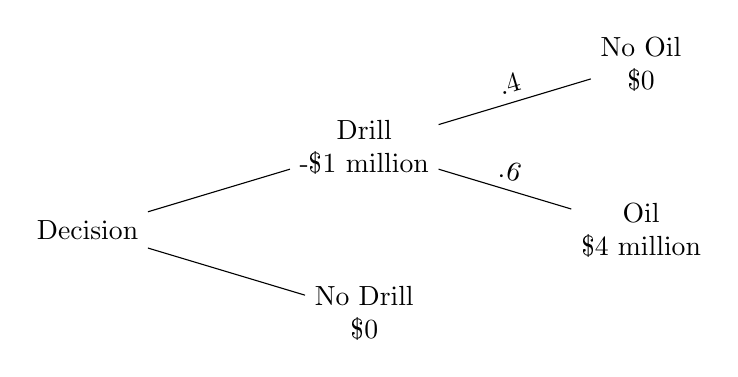
\begin{tikzpicture}
	[grow = right, sibling distance = 6em, level distance = 10em, align=center, sloped]
	%---
	\linespread{1}% <--- locally defined vertical line spacing in nodes
	%---
	\node {Decision}
	child {node {No Drill\\\$0} }
	child {node {Drill\\-\$1 million}
		child {node {Oil\\\$4 million} edge from parent node [above] {.6} }
		child {node {No Oil\\\$0} edge from parent node [above] {.4} }
		};
\end{tikzpicture}
\end{document}